\chapter{Sesnando}
\label{ch:sesnando}

This section introduces the SESNANDO project by describing the software operability and its core functionalities.

\section{Functional Overview}
%----------------------- Functional Overview ----------------------------
\label{sec:functional_overview}

This section describes how Sesnando can be used, its input resources, what the intermediate steps are and what will be generated as a result.\\
The entry point of this software is a \textit{Console application} that might take a couple of arguments. From this application \textit{Sesnando} takes the requirements defined on an input file and starts it internal processing without prompting the user. When finished, i.e., the set of test steps have been generated to validate each requirement, \textit{Sesnando} will call a Graphical User Interface (GUI) application, namely \textit{Test Designer}, to display such test steps in a Grid View. From that, the user is free to change, add or remove any test steps or signal values. The displayed test specification can be stored on a persistent file (which can be opened at any time using the \textit{Test Designer}). The user is also able to export this test specification as a test script to be used on a test execution tool or test environment.\\

The following image (Fig. \ref{fig:data_flow}) presents the main execution flow in a very simple manner. \\
\begin{figure}[H]
    \centering
    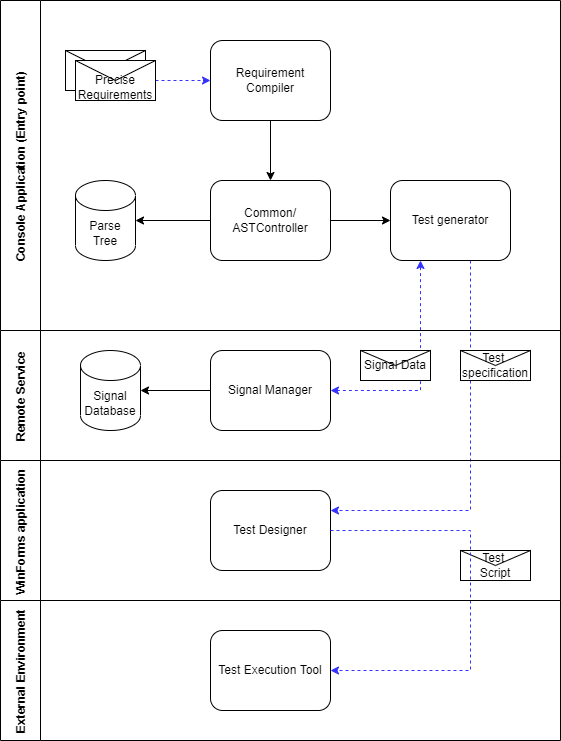
\includegraphics[scale=0.625]{images/sesnando_dataflow.png}
    \caption{Main flow diagram}
    \label{fig:data_flow}
\end{figure}

The compiler takes the requirements from the input file and parses them into an object tree by instantiating derivative classes as \textit{Logical Expressions} and stores them on the Common lib. Test Generator is then called to retrieve the object tree by asking the \textit{AST Controller} and requests the necessary information from the Signal Manager trough a \textit{Web API}. Once finished, the generated test specification is saved as a permanent file and \textit{Test Designer} is called to display such test specification to the user, as those can then be exported as a test script.